\chapter{Simulations and Analysis of the 3PWFS}

To assess the performance of the 3PWFS compared to the 4PWFS, a simulation was developed using the Object Oriented Matlab Adaptive Optics toolbox (OOMAO) \cite{OOMAO}. The OOMAO toolbox is an end-to-end adaptive optics model that can simulate different combinations of guide stars, turbulent atmospheres, wavefront sensors, deformable mirrors, and science cameras. Light is propagated using Fraunhofer diffraction. The master OOMAO toolbox simulates a 4PWFS using Slopes Maps. This chapter details the work that was done to extend OOMAO's ulitilies to include the 3PWFS and the Raw Intensity signal processing method. We then detail an experiment performed on OOMAO to study the performance of the 3PWFS compared to the 4PWFS for different magnitude guide stars. 

\section{The Object Oriented Matlab Adaptive Optics toolbox}

The OOMAO toolbox is a library of classes that are used to assemble objects that simulate different components of an adaptive optics system. The electric field is propagated object to object according to the optical path of a real AO system. The main classes include: The source class, atmosphere telescope class, deformable mirror class, pyramid class, and the detector class. The source class generates the beacon guide star used by the AO system for wavefront sensing. The guide star object contains the information of the wavelength bandpass of the system, and the user can set the magnitude of the guide star to change the intensity of light at the detector. The light from the guide star is propagated through the atmosphere to the telescope object. The atmosphere class generates the phase screens that are used to simulate turbulence. The number of layers, the wind speed, Fried parameter $r_0$, and outer and inner scale of the turbulence profile can be set. The resulting phase screens are scaled and compressed into a single phase screen in the pupil plane.  The telescope object defines the aperture of the system, the system resolution, and the exposure time. The default setting is a clear circular aperture, but central obscurations can be modeled from within OOMAO. The user can provide their own pupil mask for more complex apertures. The deformable mirror object contains the basis set used for modal wavefront sensing. In the OOMAO library there are class files to generate Zernike modes and Fourier modes. The number of actuators and the influence function of each actuator can be set by the user. For our simulations we use a Bezier influence function which is one of the provided influence functions by OOMAO. The pyramid object simulates the pyramid wavefront sensor by using a phase mask to simulate the pyramid tip. The user can select the number of facets, and the apex angle of the pyramid which sets the separation on the WFS detector. The sampling of each of the pupils and the radius of modulation are also user defined attributes to this object. The detector object records the intensity at the focal plane. At the detector the user can turn on photon noise, as well as set the read noise for the detector. 

\begin{lstlisting}[language=Python, caption=Python example]
ngs=source
\end{lstlisting}







\section{The Pyramid Object}
\subsection{The Phase Screen}
\subsection{Signal Handling}
\subsection{Calibration}





The PWFS is simulated using a single tip/tilt phase mask that is segmented into N parts. Figure \ref{fig:oomaoFigs}.A and \ref{fig:oomaoFigs}.C show the masks for the 3PWFS and 4PWFS. The masks are scaled and rotated according to a user input for rotation and pyramid apex angle that controls the separation of the pyramid pupils. After scaling, the mask is converted into a phase mask that is applied at the focal plane to simulate a pyramid tip. Figure \ref{fig:oomaoFigs}.C and \ref{fig:oomaoFigs}.D show the resulting pyramid pupils on the simulated wavefront sensor camera, using a flat wavefront and 5 $\lambda/D$ modulation. The master OOMAO toolbox simulates a 4PWFS using Slopes Maps. We extended the PWFS class in OOMAO to include a 3PWFS, taking care that the amplitude of the tip/tilt phase in the 3PWFS phase screen generation matched that of 4PWFS. We included our derivation of the Slopes Maps equation for the 3PWFS (derived in Section~\ref{SlopesDerivation} below), and added the Raw Intensity method for both the 4PWFS and the 3PWFS. For both the Slopes Maps and Raw Intensity method the signal was normalized by the mean value across all valid pixels on the wavefront sensor detector, instead of normalizing pixel by pixel. 

\begin{figure}
    \centering
    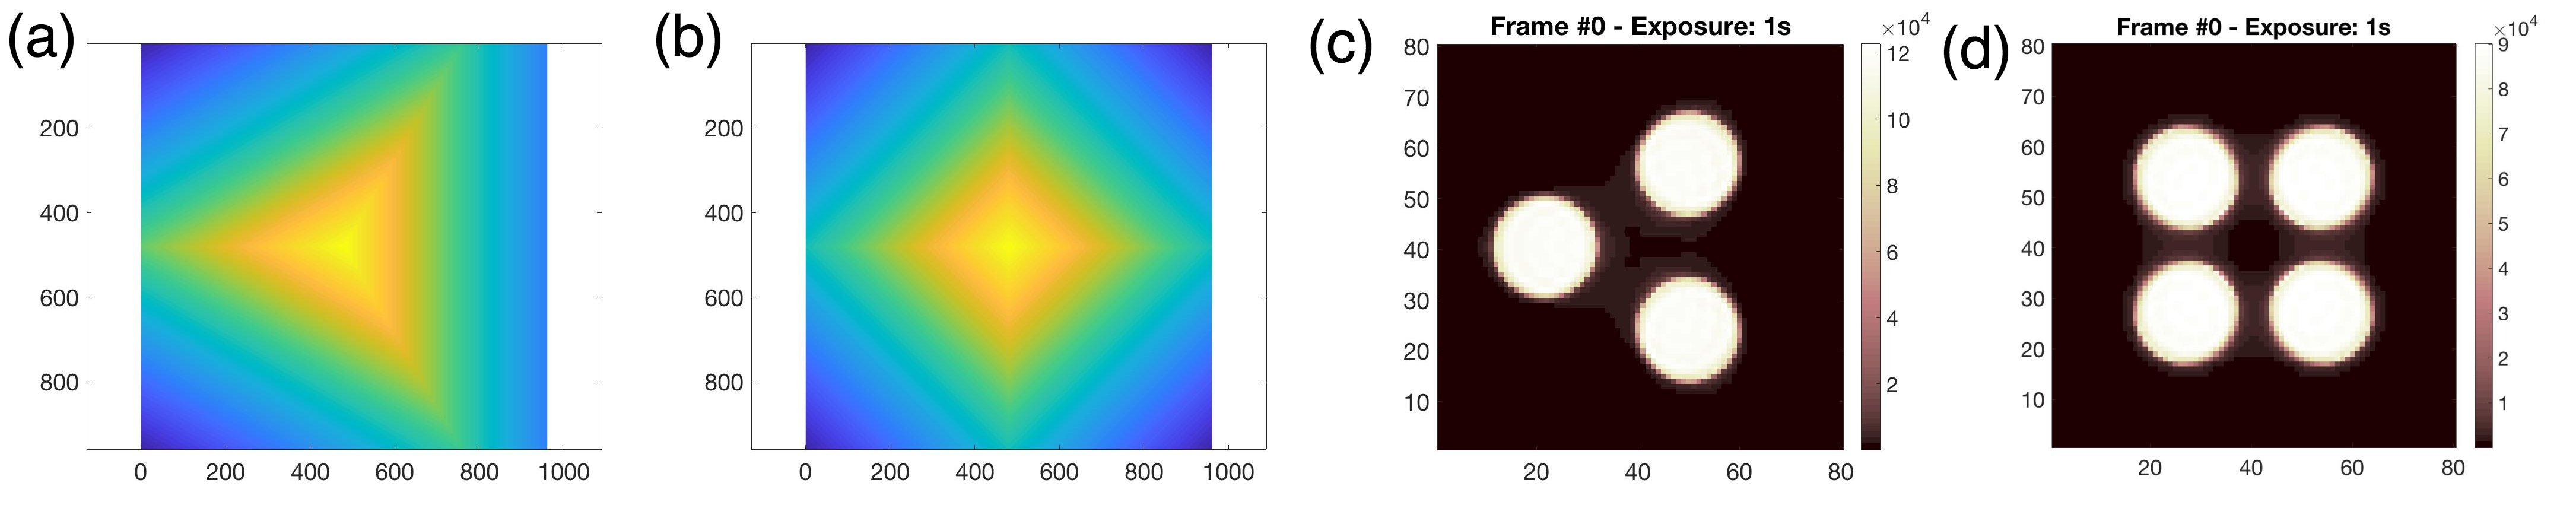
\includegraphics[width=1\textwidth]{oomaoFigs.png}
    \caption{Details of the simulated PWFS in OOMAO. A) and B) The simulated 3PWFS and 4PWFS pyramid masks in OOMAO. These masks are used as a phase screen in the pupil plane to emulate the focal plane splitting and separation done by a real glass pyramid. C) and D) The pupils from the 3PWFS and 4PWFS respectively on the simulated detector. In OOMAO the user can change the size, separation, and intensity values of the pupils through user defined inputs.}
    \label{fig:oomaoFigs}
\end{figure}


\section{Performance Comparison of the 3PWFS and 4PWFS}
\subsection{Simulation}

Using OOMAO an end to end simulation of an adaptive optics system was written to compare the performance of the 3PWFS and 4PWFS using both Raw Intensity and Slopes.  The goal was to measure the quality of correction from the AO closed loop by calculating the Strehl Ratio produced by each wavefront sensor as a function of guide star magnitude. In this simulation the Strehl ratio was calculated using OOMAO's built in Strehl calculator, which uses the OTF calculated from a PSF with no phase aberration, and a PSF with AO compensated phase aberration. The details of the simulation are summarized in the flow chart in Figure \ref{fig:simulationl}. To characterize the sensitivity of each sensor to read noise the following experiment was performed twice, once at $0.5e^-$ read noise to match that of an OCAM2K camera, and once at $12 e^-$ read noise to match the noisest camera on the Comprehensive Adaptive Optics and Coronagraph Test Instrument (CACTI) at the UA Extreme Wavefront Control Lab (XWCL). Listed below is the experiment performed in OOMAO:

\begin{itemize}
    \item Guide star magnitude was varied incrementally from 0 to 12th magnitude in steps of 2.
    \item At each magnitude closed loop data was taken with different loop gains from 0.1 to 1.8 in steps of 0.1.
    \item At each loop gain the performance was tested by closing the loop on 15 different atmospheric realizations and recording 500 closed loop PSF frames. 
    \item Strehl values were calculated from the PSFs and an average Strehl ratio is reported for a given loop gain at a given magnitude.
    \item The loop gain that gave the highest Strehl value for that guide star magnitude was used in the final calculation of Strehl vs guide star magnitude.
    \item The result is a plot of Strehl versus guide star magnitude, where the value of Strehl has been optimized over the loop gain shown in Figure \ref{fig:overall}
\end{itemize}


\begin{figure}
    \centering
    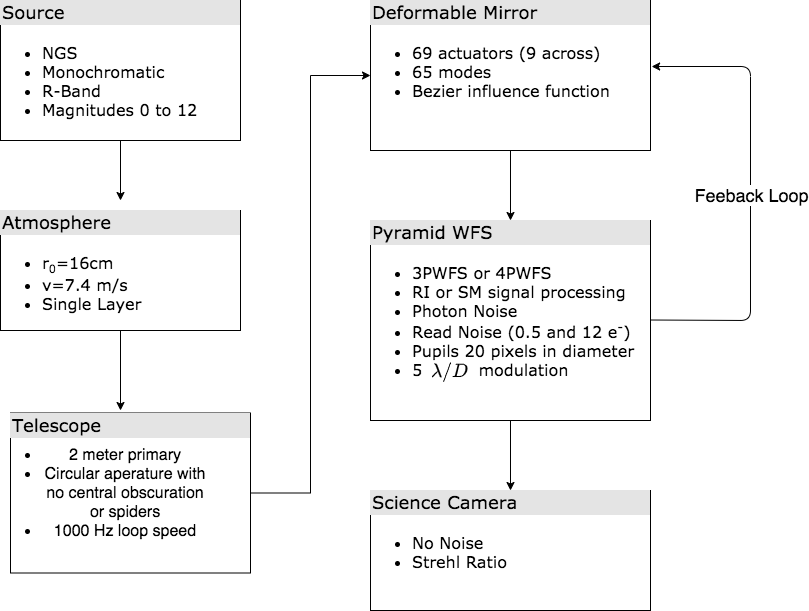
\includegraphics[width=0.8\textwidth]{simulation.png}
    \caption{Experimental details of the simulation done in OOMAO. Light starts at the natural guide star and is propagated through the atmosphere, telescope and wavefront sensor. The wavefront sensor measures a correction that is then applied by the deformable mirror.  The resulting AO corrected PSF is recorded on a noiseless science camera. }
    \label{fig:simulationl}
\end{figure}

\subsection{Results}

In Figure \ref{fig:overall}, no significant difference in performance was found in the comparison case of the wavefront sensors with 0.5$e^-$ read noise. Most on-sky adaptive optics systems use a 4PWFS with Slopes (4PWFS SM) so we use this wavefront sensor as our reference for comparison. The performance of each wavefront sensor was found to be within a percent of Strehl from the 4PWFS SM, across all stellar magnitudes. For the simulations at 12$e^-$ read noise in Figure \ref{fig:overall} a gain of 0.0359 Strehl was found for the 3PWFS using Raw Intensity (3PWFS RI) over the 4PWFS SM at a stellar magnitude of 10. At the same magnitude the 4PWFS RI also out performed the 4PWFS SM, but the gain was only 0.0122 Strehl. This simulation successfully showed the gain in performance from the 3PWFS at low light levels where the effects of read noise are stronger. The overall performance of each wavefront sensor at each guide star magnitude is given in Figure \ref{fig:overall}. In Figures \ref{fig:0RN} and \ref{fig:12RN} comparison plots were made by subtracting the Strehl values for 4PWFS SM from the other wavefront sensors, to help visualize the performance of each wavefront sensor. From these results we can conclude that the 3PWFS is a viable wavefront sensor with performance comparable to a 4PWFS.


\begin{figure}[h]
    \centering
    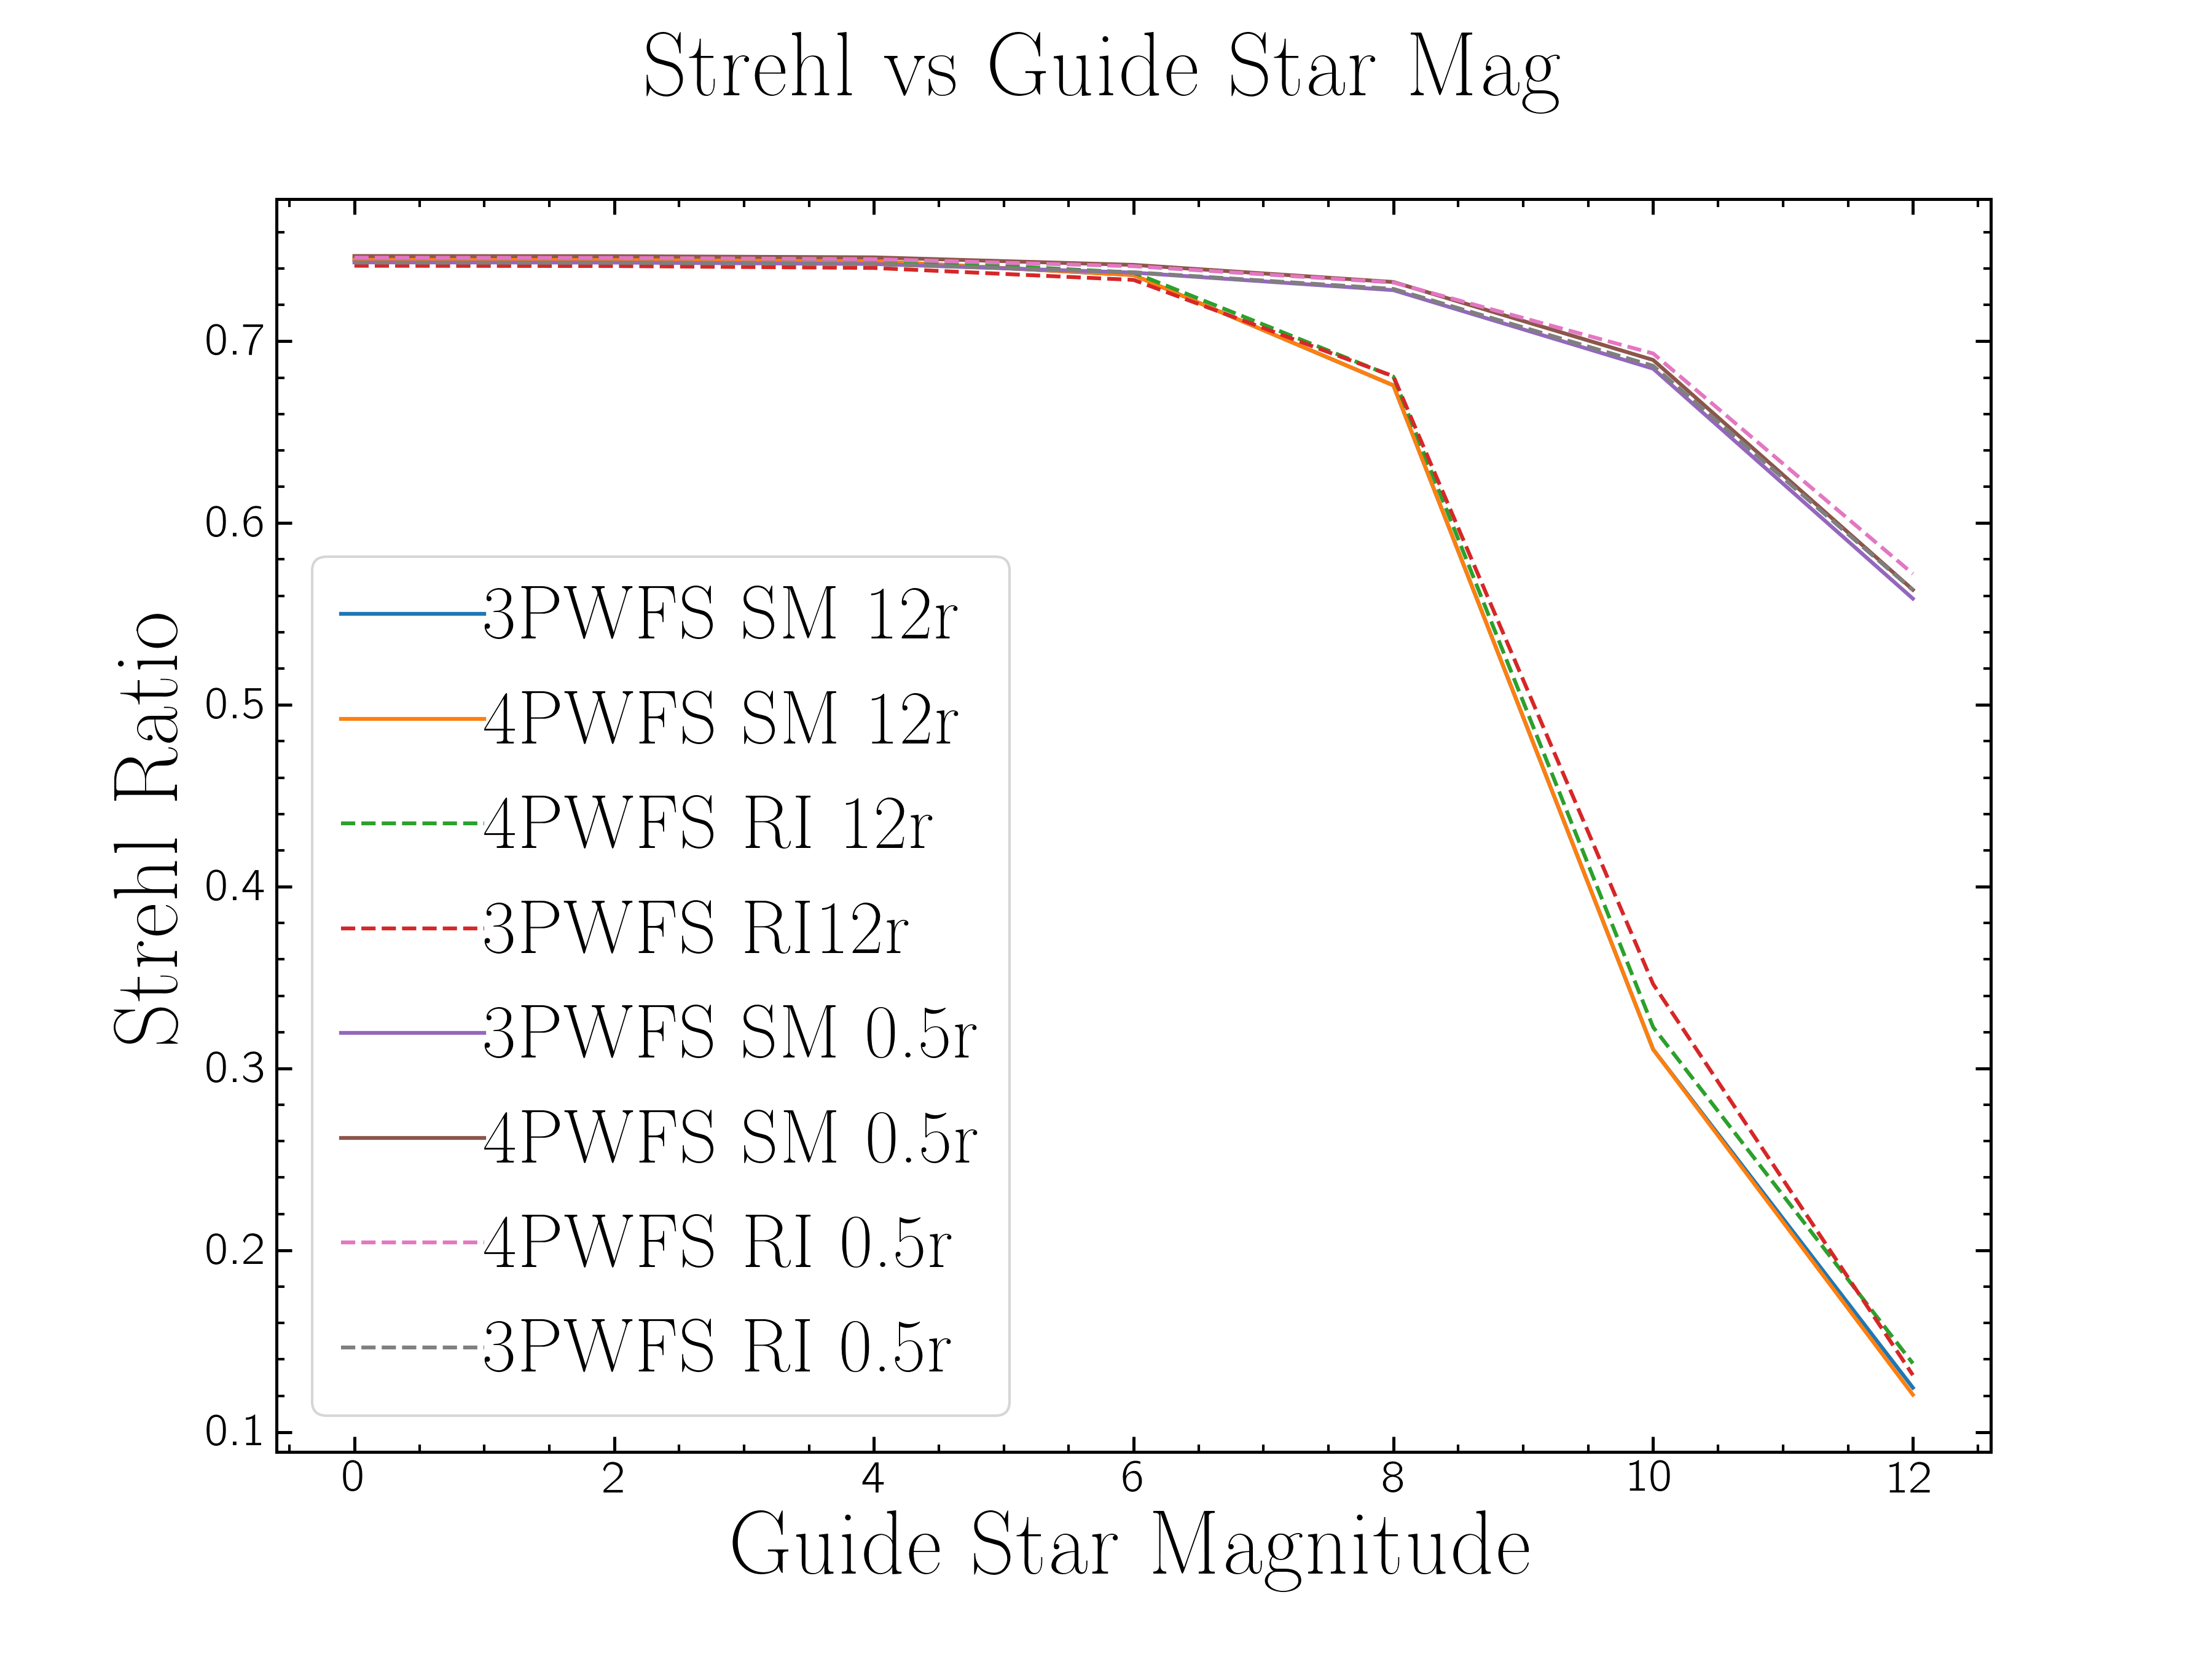
\includegraphics[width=0.8\textwidth]{StrehlvGuideStar4v3.png}
    \caption{Strehl vs Guide Star magnitude for each PWFS. The steep drop off in performance of the lower curves is due to the effects of 12$e^-$ read noise. At guide star magnitude of 10, the read noise starts to matter, and the 3PWFS out performs the 4PWFS. }
    \label{fig:overall}
\end{figure}


\begin{figure}[h]
    \centering
    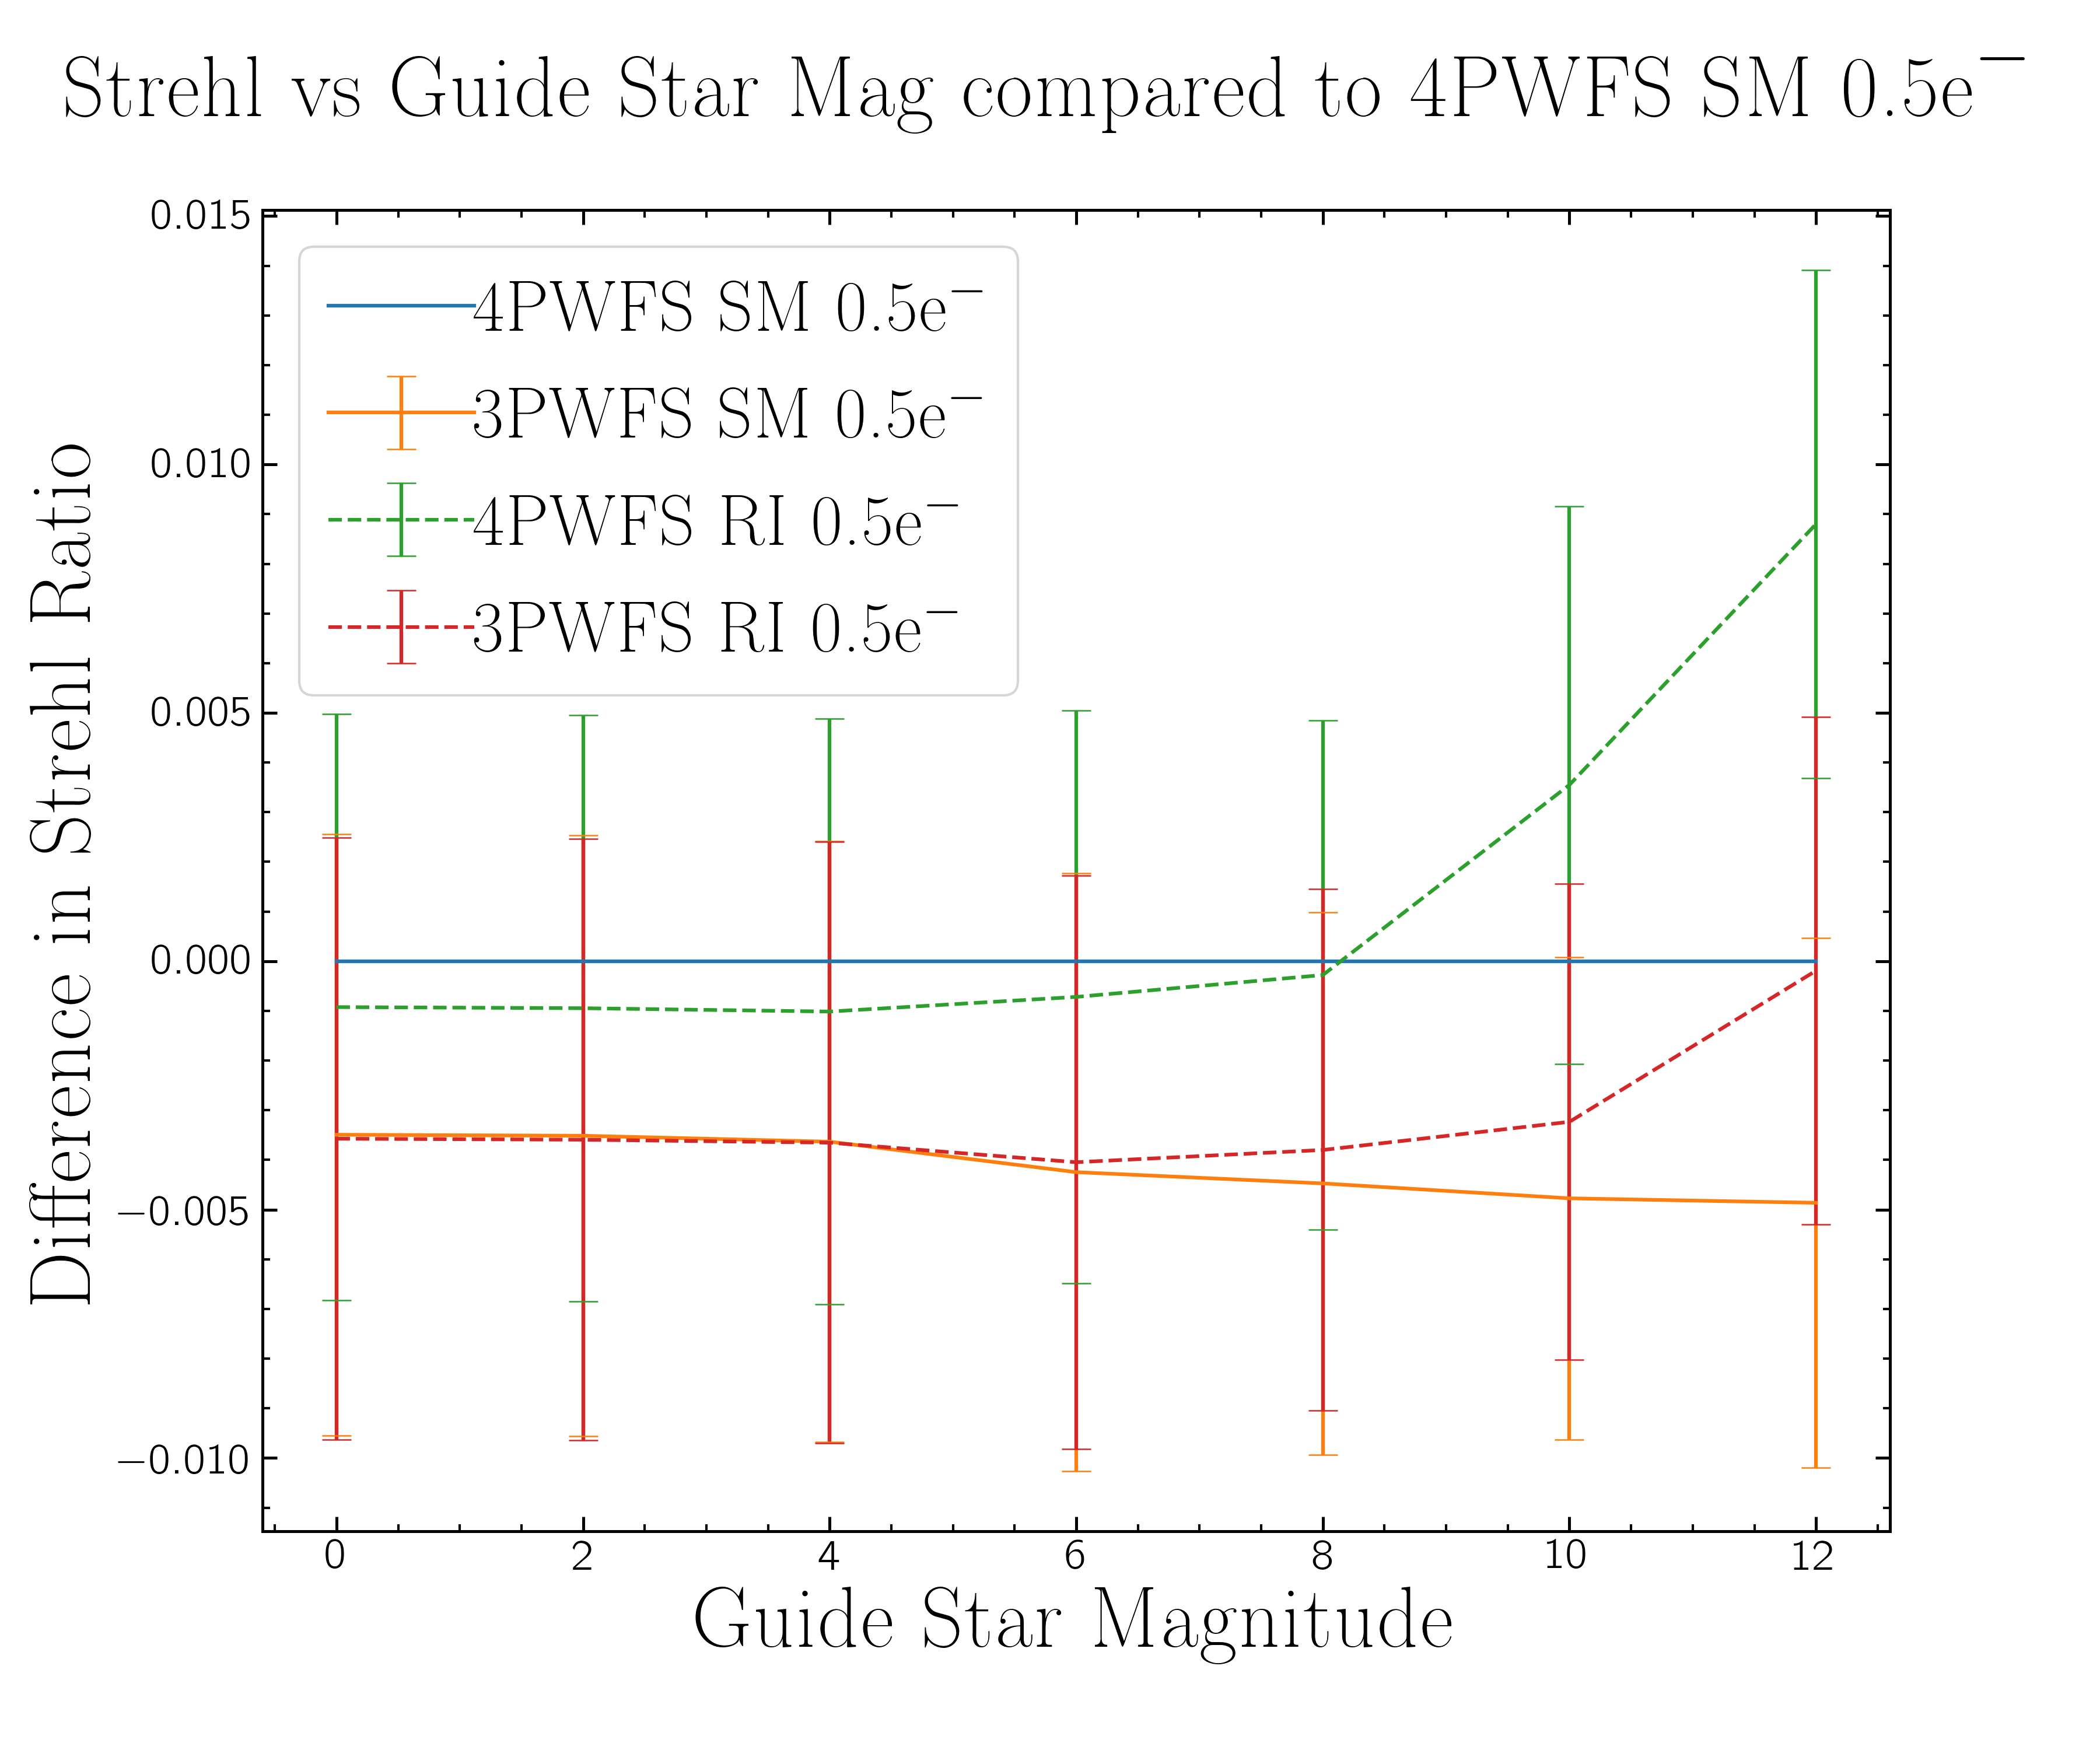
\includegraphics[width=.7\linewidth]{StrehlvGuideStarvs4PWFSRM0e.png}
    \caption{Comparison plot of wavefront sensor performance vs the 4PWFS using Slopes at 0.5 $e^-$ read noise. }
    \label{fig:0RN}
\end{figure}

\begin{figure}[h]
    \centering
    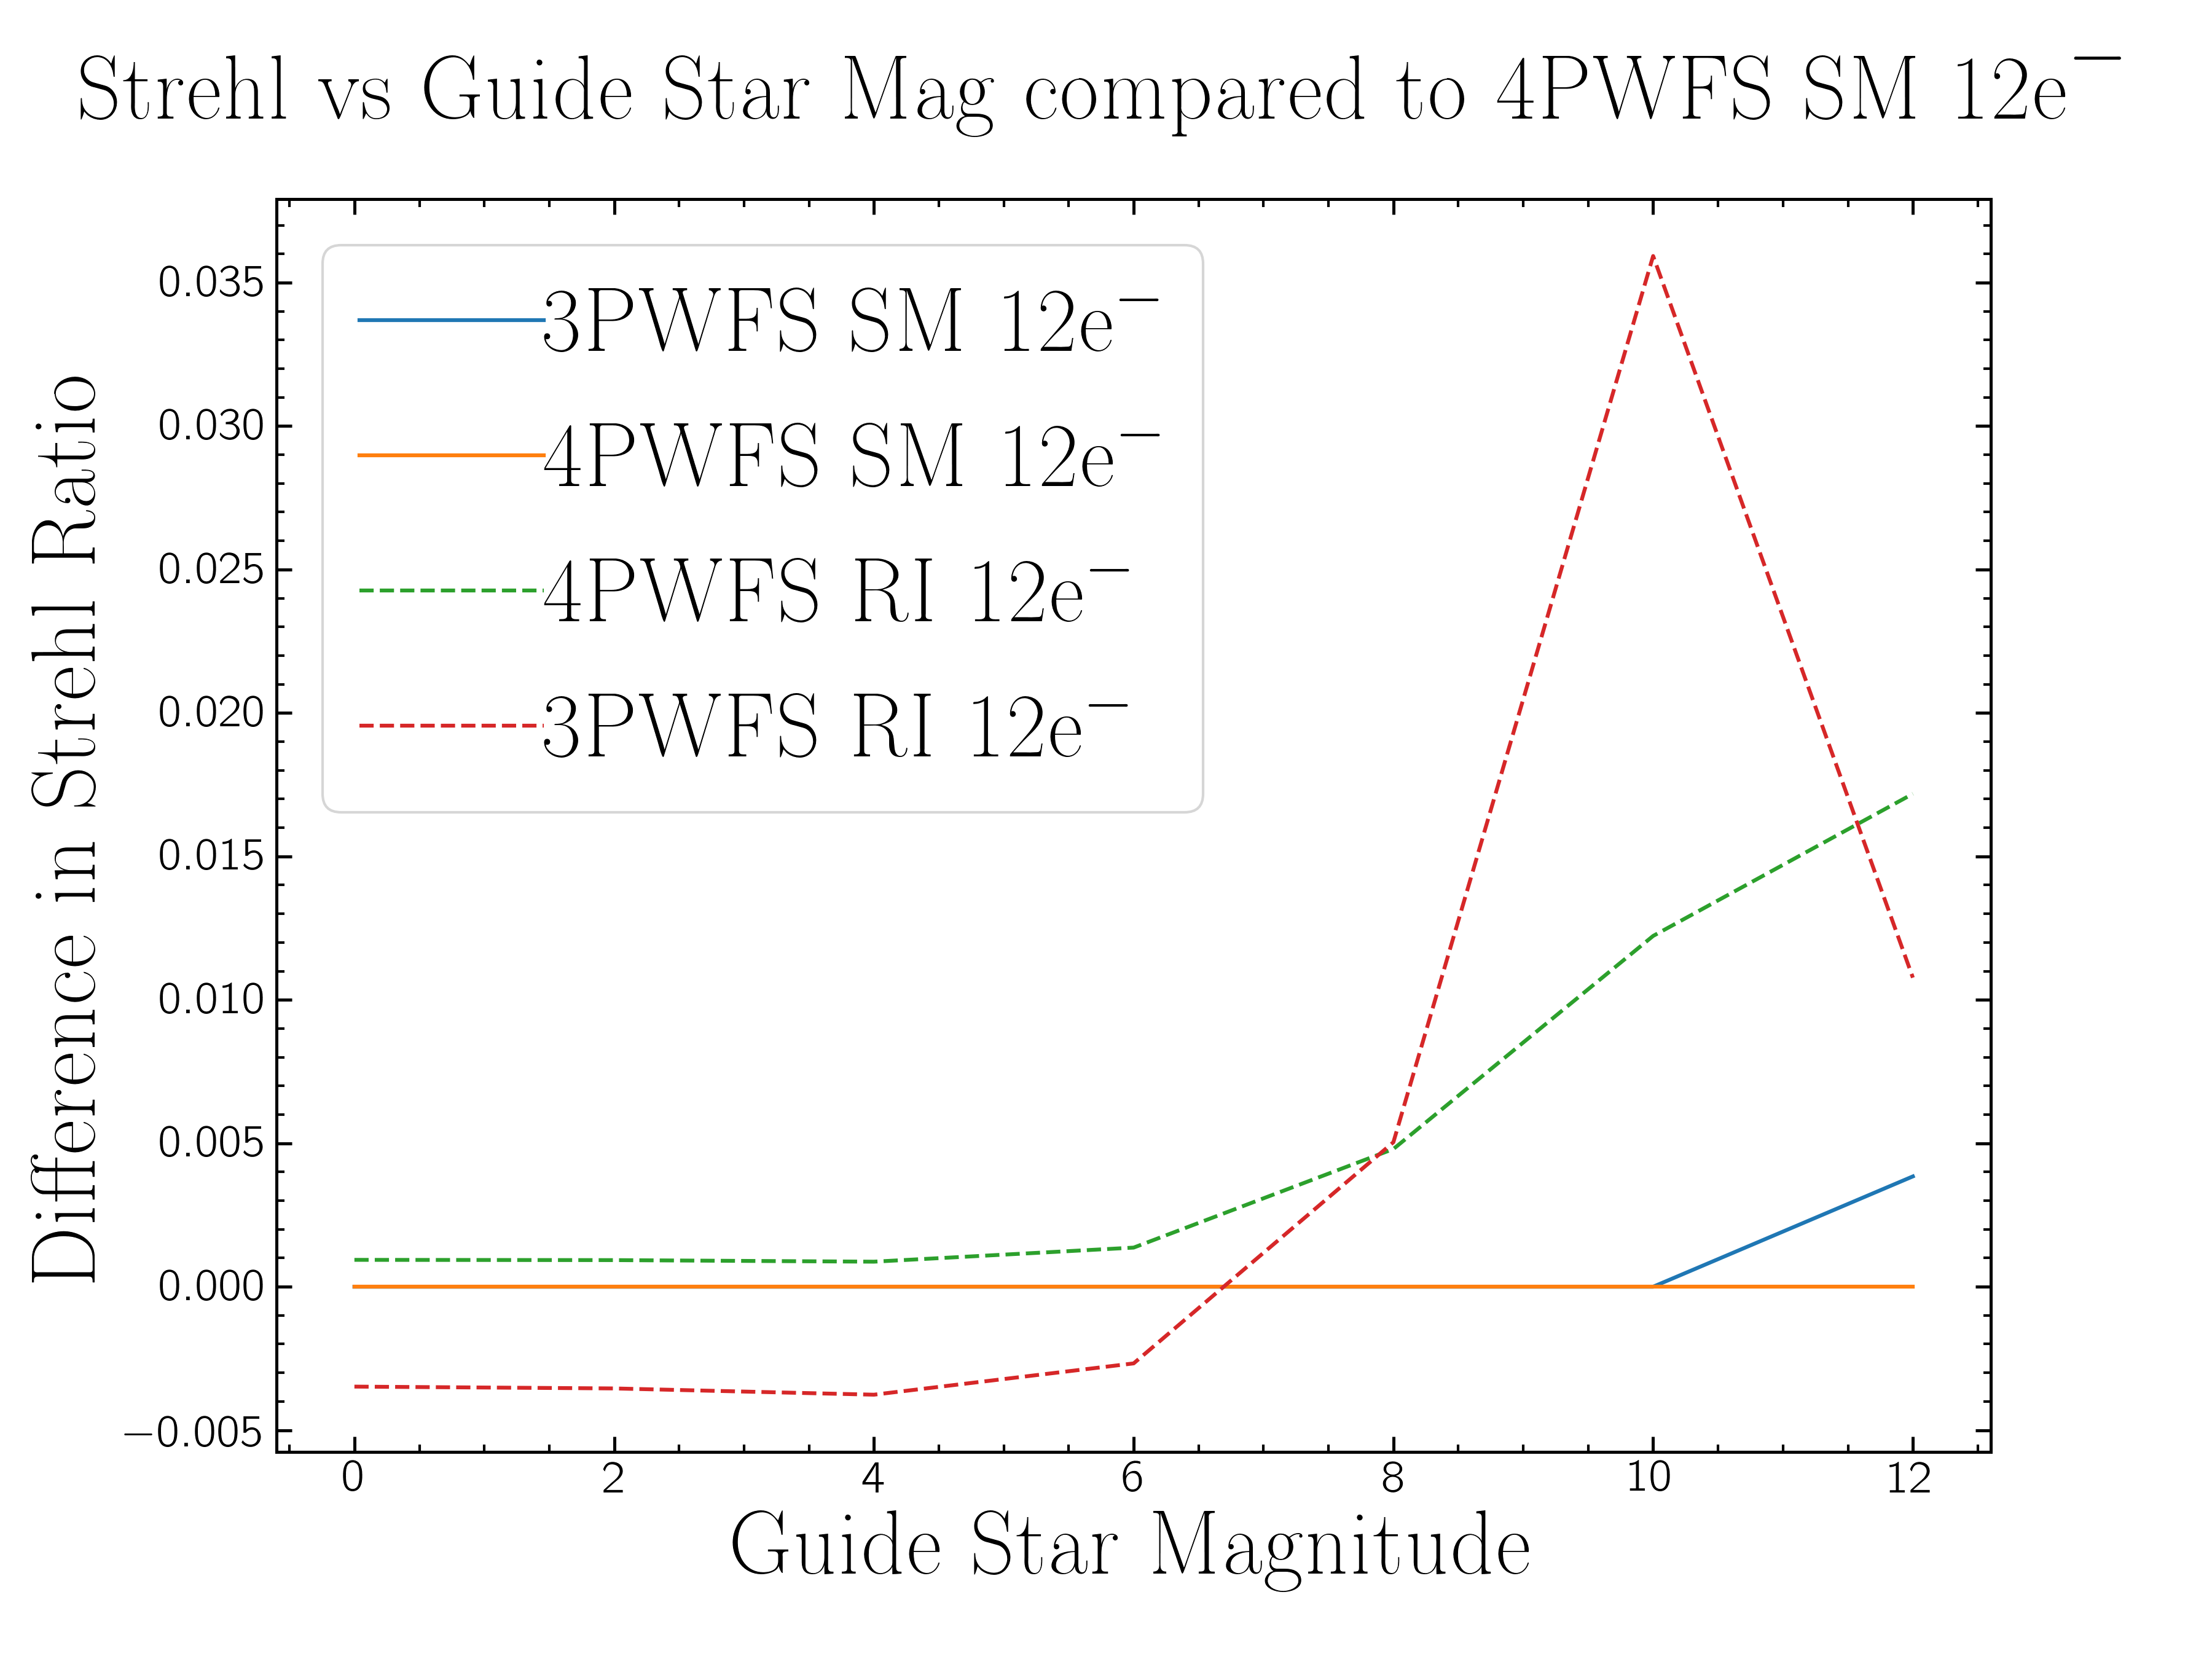
\includegraphics[width=.7\linewidth]{StrehlvGuideStarvs4PWFSRM12e.png}
    \caption{Comparison plot of wavefront sensor performance vs the 4PWFS using Slopes at 12 $e^-$ read noise.}
    \label{fig:12RN}
\end{figure}

\newpage